% =====================================================================
%  Rozdział 6 - wersja robocza do przeredagowania
%  Dane: wyniki/R6 (alarmy IDS, zbiór 60 plików, kontenery rzeczywiste),
%        wyniki/R4/r4.pcap i wyniki/R4/4.1 (nagrania ruchu)
%  Wszystkie liczby zweryfikowane z plików wyników i nagrań pcap.
%  Wykresy: tools/wykresy-praca.py r6
% =====================================================================
\chapter{Projekt i~weryfikacja wielowarstwowego systemu obronnego}\label{ch:obrona}

W rozdziale przedstawiono dwie warstwy detekcji zaprojektowane na podstawie wyników z~rozdziałów~\ref{ch:ataki} i~\ref{ch:gpu} oraz wyniki ich weryfikacji. Warstwa sieciowa wykrywa w~ruchu ślady zdarzeń zbadanych w~rozdziale~\ref{ch:ataki}: podszycie w~protokole ARP oraz zestawienie sesji TLS z~przestarzałą wersją protokołu lub słabym zestawem szyfrów. Warstwa danych rozpoznaje pliki zaszyfrowane wśród danych opuszczających organizację, co odpowiada końcowemu etapowi ataku -- wyprowadzeniu danych (ang. \ang{exfiltration}). Zaszyfrowanie lub spakowanie danych przed ich wyprowadzeniem ukrywa treść przed systemami ochrony przed wyciekiem danych (ang. \ang{Data Loss Prevention}, DLP), które analizują zawartość przesyłanych plików. Budowę systemu przedstawia rysunek~\ref{rys:warstwy}.

\begin{figure}[htbp]
\centering
\begin{tikzpicture}[
  font=\footnotesize,
  node distance=6mm and 7mm,
  warstwa/.style={draw, rounded corners=3pt, line width=0.8pt, inner xsep=6pt, inner ysep=7pt},
  blok/.style={draw, rounded corners=2pt, align=center, minimum height=11mm, text width=40mm, fill=black!4},
  wej/.style={draw, align=center, minimum height=11mm, text width=30mm},
  wyj/.style={draw, align=center, minimum height=11mm, text width=26mm, fill=black!10},
  etap/.style={draw, rounded corners=2pt, align=center, minimum height=11mm, text width=19mm, fill=black!4},
  strz/.style={-{Stealth[length=2mm]}, line width=0.7pt}
]
% --- warstwa sieciowa ---
\node[wej] (ruch) {kopia ruchu segmentu \kod{labnet} lub nagranie \kod{pcap}};
\node[blok, above right=1mm and 9mm of ruch.east, anchor=south west] (arp) {inspektor \kod{arp\_spoof}\\(wzorzec powiązań\\IP--MAC)};
\node[blok, below right=1mm and 9mm of ruch.east, anchor=north west] (tls) {reguły własne\\(sid 1000010--1000013)};
\path (arp.east |- ruch.east) ++(13mm,0) node[wyj, anchor=west] (al1) {alarmy czujnika\\(\kod{alert\_fast})};
\draw[strz] (ruch.east) -- ++(4.5mm,0) |- (arp.west);
\draw[strz] (ruch.east) -- ++(4.5mm,0) |- (tls.west);
\draw[strz] (arp.east) -- ++(4.5mm,0) |- (al1.west);
\draw[strz] (tls.east) -- ++(4.5mm,0) |- (al1.west);
\node[warstwa, fit=(ruch)(arp)(tls)(al1)] (w1) {};
\node[anchor=south west, font=\footnotesize\bfseries] at (w1.north west) {Warstwa sieciowa -- czujnik Snort~3 (podrozdział~\ref{sec:ids})};
% --- warstwa danych ---
\node[wej, below=17mm of tls.south -| ruch, anchor=north] (plik) {plik (treść opuszczająca organizację)};
\node[etap, right=6mm of plik] (h) {entropia\\$H \geq 7{,}5$};
\node[etap, right=5mm of h] (c) {$\chi^2 \leq 293{,}25$};
\node[etap, right=5mm of c] (m) {brak\\nagłówka};
\node[wyj, right=5mm of m, text width=20mm] (dec) {,,dane zaszyfrowane''};
\draw[strz] (plik) -- (h); \draw[strz] (h) -- (c); \draw[strz] (c) -- (m); \draw[strz] (m) -- (dec);
\node[warstwa, fit=(plik)(h)(c)(m)(dec)] (w2) {};
\node[anchor=south west, font=\footnotesize\bfseries] at (w2.north west) {Warstwa danych -- klasyfikator entropijny B (podrozdział~\ref{sec:entropia})};
\end{tikzpicture}
\caption{Budowa dwuwarstwowego systemu detekcji}
\label{rys:warstwy}
\end{figure}

Obie warstwy weryfikowano offline: warstwę sieciową na nagraniach ruchu zarejestrowanych przez czujnik w~trakcie eksperymentów z~rozdziału~\ref{ch:ataki}, a~warstwę danych na zbiorze plików testowych oraz na rzeczywistych plikach zaszyfrowanych utworzonych w~rozdziale~\ref{ch:gpu}. Taki sposób weryfikacji pozwala wielokrotnie uruchamiać detekcję na identycznym materiale (podrozdział~\ref{sec:czujnik}).

% ---------------------------------------------------------------------
\section{Detekcja w~warstwie sieciowej}\label{sec:ids}

\subsection*{Konfiguracja czujnika}

Detekcję w~warstwie sieciowej realizuje Snort~3.12.2.0~\cite{snort3} na maszynie \kod{sensor} -- otwarty system IDS, którego właściwości porównano z~systemem Suricata m.in. w~pracy~\cite{boukebous2023}. Ustawienia laboratorium (plik \kod{lab.lua}) obejmują trzy elementy:
\begin{itemize}
  \item zmienną \kod{HOME\_NET} ustawioną na sieć laboratorium 10.10.10.0/24;
  \item inspektor \kod{arp\_spoof} ze wzorcem powiązań adresów IP i~MAC klienta oraz serwera (tabela~\ref{tab:arp-wzorzec});
  \item włączone reguły wbudowane, do których należą alarmy inspektora \kod{arp\_spoof} (identyfikator generatora 112), oraz dołączony plik reguł własnych \kod{local.rules}.
\end{itemize}

Reguły własne wykrywają w~komunikacie ServerHello, wysyłanym przez serwer w~odpowiedzi na ofertę klienta, wersję protokołu i~zestaw szyfrów wybrane przez serwer. Komunikat ten jest przesyłany jawnie we wszystkich wersjach protokołu, również w~TLS~1.3. Położenie pól wykorzystywanych przez reguły podano w~tabeli~\ref{tab:serverhello}.

\begin{table}[htbp]
\centering\small
\begin{tabularx}{\textwidth}{@{}l l L@{}}
\toprule
\textbf{Bajty} & \textbf{Pole} & \textbf{Wartość wykorzystywana w~regułach} \\
\midrule
0       & typ rekordu TLS & \kod{0x16} (rekord uzgadniania) \\
1--2    & wersja rekordu & \kod{0x03 0xXX} \\
3--4    & długość rekordu & -- \\
5       & typ komunikatu & \kod{0x02} (ServerHello) \\
6--8    & długość komunikatu & -- \\
9--10   & wersja protokołu wybrana przez serwer & \kod{0x0300} -- SSLv3, \kod{0x0301} -- TLS~1.0, \kod{0x0302} -- TLS~1.1 \\
11--42  & wartość losowa serwera (32~B) & -- \\
43      & długość identyfikatora sesji ($n$) & -- \\
44+$n$, 45+$n$ & wybrany zestaw szyfrów & \kod{0xC014} -- \kod{ECDHE-RSA-AES256-SHA} \\
\bottomrule
\end{tabularx}
\caption{Pola komunikatu ServerHello liczone od początku rekordu TLS}
\label{tab:serverhello}
\end{table}

Reguły wersji (sid 1000010--1000012) sprawdzają kolejno: typ rekordu, typ komunikatu i~wartość pola wersji. W~TLS~1.3 pole to zawiera zawsze wartość \kod{0x0303}, a~rzeczywista wersja jest przenoszona w~rozszerzeniu \ang{supported\_versions}. Wartości \kod{0x0303} nie można więc użyć do odróżnienia TLS~1.2 od TLS~1.3 i~reguły celowo pomijają ją, ograniczając się do wartości oznaczających wersje przestarzałe: SSLv3, TLS~1.0 i~TLS~1.1, z~których dwie ostatnie formalnie wycofał RFC~8996~\cite{rfc8996}. Reguła słabego szyfru (sid 1000013) szuka bajtów \kod{0xC014} w~oknie zaczynającym się 30~bajtów za polem typu komunikatu, czyli od 36. bajtu rekordu. Położenie zestawu szyfrów zależy od długości identyfikatora sesji; w~badanym nagraniu reguła dopasowała go zarówno na pozycji 44 (identyfikator pusty), jak i~76 (identyfikator 32-bajtowy). Okno obejmuje także końcówkę pola losowego i~identyfikator sesji, dlatego reguła jest heurystyką: przypadkowe wystąpienie tych bajtów w~polach losowych spowodowałoby fałszywy alarm. Treść reguł przedstawia listing~\ref{lst:reguly}; reguły 1000011 i~1000012 różnią się od 1000010 wyłącznie treścią komunikatu i~szukaną wartością wersji (\kod{|03 01|}, \kod{|03 02|}).

\begin{lstlisting}[float=htbp, caption={Reguły własne czujnika do wykrywania przestarzałych parametrów sesji TLS (fragment pliku \kod{local.rules})}, label={lst:reguly}]
alert tcp any any -> any any ( msg:"LAB 6.1 - ServerHello: wynegocjowano SSLv3 (przestarzaly protokol)";
    flow:to_client,established;
    content:"|16 03|", offset 0, depth 2;
    content:"|02|", offset 5, depth 1;
    content:"|03 00|", offset 9, depth 2;
    sid:1000010; rev:1; )

alert tcp any any -> any any ( msg:"LAB 6.1 - ServerHello: wynegocjowano slaby szyfr ECDHE-RSA-AES256-SHA (CBC/SHA1)";
    flow:to_client,established;
    content:"|16 03|", offset 0, depth 2;
    content:"|02|", offset 5, depth 1;
    content:"|c0 14|", distance 30, within 60;
    sid:1000013; rev:1; )
\end{lstlisting}

\subsection*{Materiał testowy}

Reguły i~inspektor uruchomiono offline na nagraniu \kod{r4.pcap}, zarejestrowanym przez czujnik 25.10.2026 w~czasie eksperymentów z~podrozdziałów~\ref{sec:tlsneg}--\ref{sec:lenext}. Nagranie trwa około 34~minut (2064~s) i~zawiera 10\,261 pakietów, w~tym:
\begin{itemize}
  \item 15 komunikatów ServerHello obu serwerów: po 7 z~dwóch przebiegów skanu wersji protokołu (podrozdział~\ref{sec:tlsneg}) i~jeden z~dodatkowego połączenia TLS~1.3 z~serwerem utwardzonym, zarejestrowanego między przebiegami;
  \item 827 żądań HTTP \kod{GET} do aplikacji testowej (10.10.10.30, port 5000) z~eksperymentów dotyczących integralności;
  \item 8 ramek ARP -- cztery pary zapytanie--odpowiedź wymieniane przez klienta i~serwer w~trakcie zwykłej pracy; wszystkie zawierają poprawne powiązania adresów, zgodne ze wzorcem.
\end{itemize}
Nagranie nie zawiera zatem żadnej próby podszycia w~ARP. Detekcję takiej próby zweryfikowano na osobnym nagraniu \kod{arp41.pcap} z~podrozdziału~\ref{sec:arp}.

\subsection*{Wyniki}

Na nagraniu \kod{r4.pcap} czujnik zgłosił 15~alarmów: 12 z~reguł własnych i~3 z~inspektora \kod{arp\_spoof}. Alarmy reguł własnych przedstawia rysunek~\ref{rys:snort-tls}, a~ich przyporządkowanie do poszczególnych komunikatów ServerHello -- tabela~\ref{tab:ids-serverhello}. Zestaw szyfrów każdego komunikatu odczytano bezpośrednio z~nagrania.

\begin{figure}[htbp]
\centering
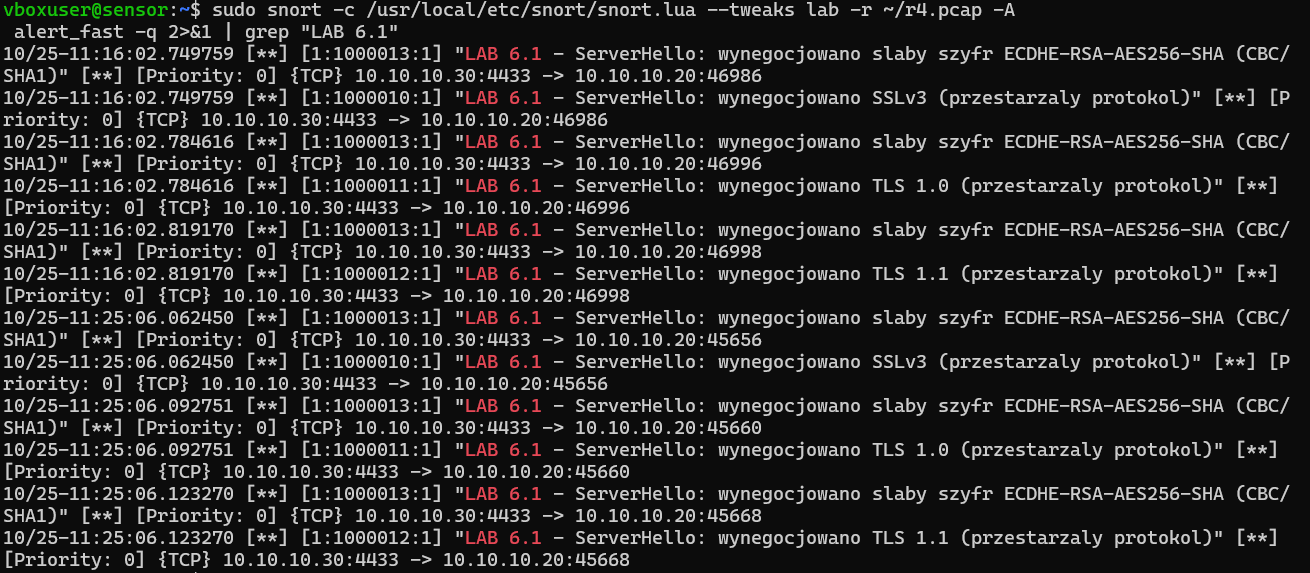
\includegraphics[width=\textwidth]{rysunki/r6-snort-tls.png}
\caption{Alarmy reguł własnych na nagraniu \kod{r4.pcap} (wyjście programu Snort przefiltrowane do reguł ,,LAB 6.1'')}
\label{rys:snort-tls}
\end{figure}

\begin{table}[htbp]
\centering\small
\begin{tabularx}{\textwidth}{@{}l l L c l@{}}
\toprule
\textbf{Serwer} & \textbf{Wersja} & \textbf{Zestaw szyfrów} & \textbf{Liczba} & \textbf{Alarmy (sid)} \\
\midrule
:443  & TLS~1.2 & \kod{ECDHE-RSA-AES128-GCM-SHA256} (\kod{0xC02F}) & 2 & brak \\
:443  & TLS~1.3 & \kod{TLS\_AES\_256\_GCM\_SHA384} (\kod{0x1302}) & 3 & brak \\
:4433 & SSLv3   & \kod{ECDHE-RSA-AES256-SHA} (\kod{0xC014}) & 2 & 1000010, 1000013 \\
:4433 & TLS~1.0 & \kod{ECDHE-RSA-AES256-SHA} (\kod{0xC014}) & 2 & 1000011, 1000013 \\
:4433 & TLS~1.1 & \kod{ECDHE-RSA-AES256-SHA} (\kod{0xC014}) & 2 & 1000012, 1000013 \\
:4433 & TLS~1.2 & \kod{ECDHE-RSA-AES256-GCM-SHA384} (\kod{0xC030}) & 4 & brak \\
\midrule
\multicolumn{3}{@{}l}{\textbf{Razem}} & \textbf{15} & \textbf{12 alarmów} \\
\bottomrule
\end{tabularx}
\caption{Komunikaty ServerHello w~nagraniu \kod{r4.pcap} i~wywołane przez nie alarmy}
\label{tab:ids-serverhello}
\end{table}

Każdy z~sześciu komunikatów z~przestarzałą wersją protokołu wywołał alarm reguły wersji (po dwa dla SSLv3, TLS~1.0 i~TLS~1.1) i~alarm reguły słabego szyfru, ponieważ we wszystkich tych sesjach serwer wybrał zestaw \kod{ECDHE-RSA-AES256-SHA}. Dziewięć pozostałych komunikatów -- wszystkie z~serwera utwardzonego oraz sesje TLS~1.2 serwera przestarzałego z~zestawem AEAD -- nie wywołało żadnego alarmu. Reguły własne wykryły więc 6 z~6 sesji z~przestarzałymi parametrami, nie zgłaszając żadnego fałszywego alarmu dla 9 sesji poprawnych. Heurystyczne okno reguły 1000013 nie spowodowało w~nagraniu przypadkowych dopasowań: bajty \kod{0xC014} wystąpiły w~danych komunikatów ServerHello wyłącznie w~polu zestawu szyfrów.

Trzy alarmy inspektora \kod{arp\_spoof} to alarmy o~identyfikatorze 112:1 (,,\ang{unicast ARP request}''). Ich znaczniki czasu odpowiadają dokładnie trzem zapytaniom ARP w~nagraniu, które zostały wysłane bezpośrednio na znany adres sprzętowy odbiorcy zamiast na adres rozgłoszeniowy (tabela~\ref{tab:ids-arp}). Zapytania takie wysyła system Linux przy sprawdzaniu aktualności wpisu w~tablicy sąsiadów, a~klient i~serwer pracują pod kontrolą systemu Ubuntu. Wszystkie trzy zawierały poprawne powiązania adresów, są to więc fałszywe alarmy.

\begin{table}[htbp]
\centering\small
\begin{tabularx}{\textwidth}{@{}r l l l L@{}}
\toprule
\textbf{Czas [s]} & \textbf{Operacja} & \textbf{Nadawca} & \textbf{Adresat ramki} & \textbf{Alarm} \\
\midrule
27,679  & zapytanie  & 10.10.10.20 & rozgłoszeniowy & brak \\
27,680  & odpowiedź  & 10.10.10.30 & 10.10.10.20 & brak \\
341,735 & zapytanie  & 10.10.10.20 & 10.10.10.30 (unicast) & 112:1 \\
341,736 & odpowiedź  & 10.10.10.30 & 10.10.10.20 & brak \\
341,926 & zapytanie  & 10.10.10.30 & 10.10.10.20 (unicast) & 112:1 \\
341,927 & odpowiedź  & 10.10.10.20 & 10.10.10.30 & brak \\
576,669 & zapytanie  & 10.10.10.30 & 10.10.10.20 (unicast) & 112:1 \\
576,670 & odpowiedź  & 10.10.10.20 & 10.10.10.30 & brak \\
\bottomrule
\end{tabularx}
\caption{Ramki ARP w~nagraniu \kod{r4.pcap} (czas od początku nagrania; wszystkie powiązania zgodne ze wzorcem)}
\label{tab:ids-arp}
\end{table}

Zestawienie skuteczności warstwy sieciowej na obu nagraniach zawiera tabela~\ref{tab:ids-bilans}. W~nagraniu \kod{r4.pcap} trafnych było 12 z~15~alarmów. Wszystkie alarmy fałszywe pochodziły z~alarmu 112:1, który zgłasza każde zapytanie typu unicast, niezależnie od tego, czy zawarte w~nim powiązanie jest poprawne. Alarmy 112:3 i~112:4, które wskazały próbę podszycia w~podrozdziale~\ref{sec:arp}, na zwykłym ruchu nie wystąpiły ani razu.

\begin{table}[htbp]
\centering\small
\begin{tabularx}{\textwidth}{@{}L l c c@{}}
\toprule
\textbf{Zdarzenie} & \textbf{Nagranie} & \textbf{Wykryte} & \textbf{Fałszywe alarmy} \\
\midrule
podszycie w~ARP (alarmy 112:3, 112:4) & \kod{arp41.pcap} & 3 z~3 ramek & 0 (3 ogłoszenia) \\
zwykły ruch ARP (alarm 112:1) & \kod{r4.pcap} & -- & 3 (z~8 ramek) \\
przestarzała wersja TLS (1000010--1000012) & \kod{r4.pcap} & 6 z~6 sesji & 0 (z~9 sesji) \\
słaby zestaw szyfrów (1000013) & \kod{r4.pcap} & 6 z~6 sesji & 0 (z~9 sesji) \\
\bottomrule
\end{tabularx}
\caption{Skuteczność warstwy sieciowej}
\label{tab:ids-bilans}
\end{table}

% ---------------------------------------------------------------------
\section{Detekcja prób eksfiltracji na podstawie analizy entropii}\label{sec:entropia}

\subsection*{Cechy i~klasyfikatory}

Warstwa danych ocenia, czy plik zawiera dane zaszyfrowane, na podstawie rozkładu wartości jego bajtów. Wykorzystywane są trzy cechy:
\begin{itemize}
  \item \textbf{entropia Shannona} $H = -\sum_{i=0}^{255} p_i \log_2 p_i$, gdzie $p_i$ to udział bajtów o~wartości~$i$; wynosi od 0 do 8~bitów na bajt, a~wartość bliską 8 mają dane o~rozkładzie zbliżonym do losowego~\cite{davies2022};
  \item \textbf{statystyka chi-kwadrat} $\chi^2 = \sum_{i=0}^{255} (n_i - E)^2 / E$, gdzie $n_i$ to liczba bajtów o~wartości~$i$, a~$E = N/256$ to liczba oczekiwana przy rozkładzie jednostajnym dla pliku o~długości $N$; mierzy odstępstwo rozkładu od jednostajnego;
  \item \textbf{rozpoznany nagłówek} -- obecność na początku pliku sygnatury znanego formatu (gzip, zip, 7z, PNG, JPEG, PDF, bzip2, xz, RAR).
\end{itemize}

Porównano dwa klasyfikatory, dla których klasą pozytywną są dane zaszyfrowane:
\begin{itemize}
  \item \textbf{klasyfikator A} -- plik jest zaszyfrowany, jeżeli $H \geq 7{,}5$;
  \item \textbf{klasyfikator B} -- plik jest zaszyfrowany, jeżeli $H \geq 7{,}5$, $\chi^2 \leq 293{,}25$ i~nie rozpoznano nagłówka.
\end{itemize}
Próg $\chi^2$ to kwantyl rzędu 0,95 rozkładu chi-kwadrat o~255 stopniach swobody (293,248). Dla danych o~rozkładzie jednostajnym statystyka $\chi^2$ przekracza ten próg z~prawdopodobieństwem około 5\%. Obliczenia wykonują skrypty \kod{r6-entropia.py} (zbiór testowy) i~\kod{r6-realne.py} (pliki rzeczywiste), napisane w~języku Python z~użyciem wyłącznie biblioteki standardowej.

\subsection*{Zbiór testowy}

Zbiór testowy wygenerował skrypt \kod{r6-gen-zbior.py}. Zawiera on 60 plików w~trzech grupach po 20 (tabela~\ref{tab:zbior}). Treść plików jawnych i~rozmiary plików zaszyfrowanych wyznacza generator pseudolosowy o~stałym ziarnie 20261029. Zawartość plików zaszyfrowanych pochodzi z~systemowego generatora liczb losowych (\kod{os.urandom}), który modeluje wynik działania dobrego szyfru; nie jest ona odtwarzalna bit po bicie.

\begin{table}[htbp]
\centering\small
\begin{tabularx}{\textwidth}{@{}l L r@{}}
\toprule
\textbf{Grupa} & \textbf{Zawartość} & \textbf{Rozmiar [B]} \\
\midrule
jawne (20) & tekst, kod w~języku Python, CSV, JSON, dziennik serwera, HTML -- po kolei & 6\,189--39\,287 \\
skompresowane (20) & pliki jawne po kompresji: gzip (10 plików) i~zip (10 plików), stopień kompresji 9 & 740--9\,084 \\
zaszyfrowane (20) & dane losowe bez nagłówka & 8\,573--62\,991 \\
\bottomrule
\end{tabularx}
\caption{Skład zbioru testowego}
\label{tab:zbior}
\end{table}

\subsection*{Wyniki}

Średnie wartości cech oraz ich zakresy w~grupach podano w~tabeli~\ref{tab:cechy}, a~położenie wszystkich plików w~przestrzeni cech -- na rysunku~\ref{rys:rozrzut}. Pliki skompresowane i~zaszyfrowane mają zbliżoną, wysoką entropię, a~ich zakresy niemal się stykają: najwyższa entropia pliku skompresowanego wynosi 7,9778, a~najniższa pliku zaszyfrowanego -- 7,9780~bitu na bajt. Rozdzielenie tych grup samą entropią wymagałoby więc progu dobranego z~dokładnością do 0,0002~bitu na bajt pod ten konkretny zbiór, co nie ma praktycznego znaczenia; trudność odróżnienia danych skompresowanych od zaszyfrowanych na podstawie entropii opisano również w~literaturze~\cite{degaspari2022}. Grupy różnią się natomiast statystyką $\chi^2$: wszystkie pliki zaszyfrowane leżą poniżej progu, a~większość plików skompresowanych -- powyżej.

\begin{table}[htbp]
\centering\small
\begin{tabular}{@{}lrrrr@{}}
\toprule
\textbf{Grupa} & \textbf{Średnia $H$} & \textbf{Zakres $H$} & \textbf{Średnia $\chi^2$} & \textbf{Zakres $\chi^2$} \\
\midrule
jawne         & 4,331 & 3,8582--4,6308 & 439\,854,8 & 124\,783,8--726\,731,3 \\
skompresowane & 7,815 & 7,2486--7,9778 & 575,0      & 251,3--1\,636,9 \\
zaszyfrowane  & 7,994 & 7,9780--7,9972 & 257,3      & 223,4--284,3 \\
\bottomrule
\end{tabular}
\caption{Entropia [bit/bajt] i~statystyka $\chi^2$ w~grupach zbioru testowego}
\label{tab:cechy}
\end{table}

\begin{figure}[htbp]
\centering
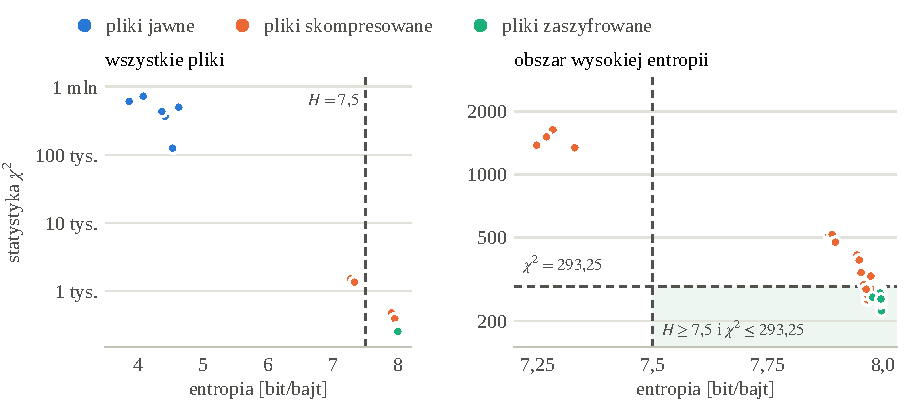
\includegraphics[width=\textwidth]{rysunki/r6-rozrzut.pdf}
\caption{Pliki zbioru testowego w~przestrzeni cech; prawy panel powiększa obszar wysokiej entropii, zacieniowano obszar spełniający oba progi klasyfikatora B}
\label{rys:rozrzut}
\end{figure}

Działanie kolejnych warunków klasyfikatora B przedstawia rysunek~\ref{rys:etapy}. Warunek entropii odrzucił wszystkie pliki jawne oraz cztery najmniejsze archiwa zip (740--751~B), przepuszczając 16 plików skompresowanych. Warunek $\chi^2$ odrzucił 11 z~nich. Pozostałe 5 plików to archiwa gzip, których statystyka $\chi^2$ nie przekroczyła progu (251,3--283,4); odrzuciło je dopiero rozpoznanie nagłówka. Wszystkie 20 plików zaszyfrowanych spełniło wszystkie trzy warunki.

\begin{figure}[htbp]
\centering
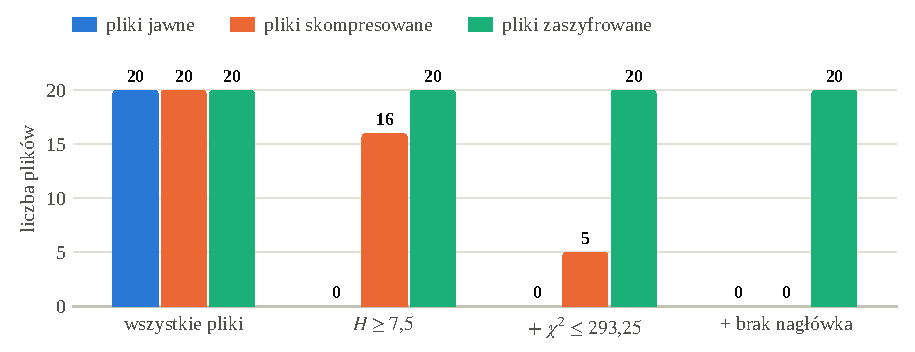
\includegraphics[width=\textwidth]{rysunki/r6-etapy.pdf}
\caption{Liczba plików uznanych za zaszyfrowane po kolejnych warunkach klasyfikatora B}
\label{rys:etapy}
\end{figure}

Macierze pomyłek i~miary jakości obu klasyfikatorów zawiera tabela~\ref{tab:klasyfikatory}, a~wynik działania skryptu -- rysunek~\ref{rys:entropia}. Klasyfikator A wykrył wszystkie pliki zaszyfrowane, ale uznał za zaszyfrowane także 16 z~20 plików skompresowanych, co daje 40\% fałszywych alarmów wśród 40 plików niezaszyfrowanych. Klasyfikator B rozpoznał wszystkie pliki poprawnie.

\begin{table}[htbp]
\centering\small
\begin{tabular}{@{}lcc@{}}
\toprule
\textbf{Miara} & \textbf{Klasyfikator A} & \textbf{Klasyfikator B} \\
\midrule
prawdziwie pozytywne (TP)  & 20 & 20 \\
fałszywie pozytywne (FP)   & 16 & 0 \\
prawdziwie negatywne (TN)  & 24 & 40 \\
fałszywie negatywne (FN)   & 0  & 0 \\
\midrule
czułość, TP/(TP+FN)                 & 100,0\% & 100,0\% \\
odsetek fałszywych alarmów, FP/(FP+TN) & 40,0\% & 0,0\% \\
precyzja, TP/(TP+FP)                & 55,6\%  & 100,0\% \\
dokładność, (TP+TN)/60              & 73,3\%  & 100,0\% \\
\bottomrule
\end{tabular}
\caption{Macierze pomyłek i~miary jakości klasyfikatorów na zbiorze testowym}
\label{tab:klasyfikatory}
\end{table}

\begin{figure}[htbp]
\centering
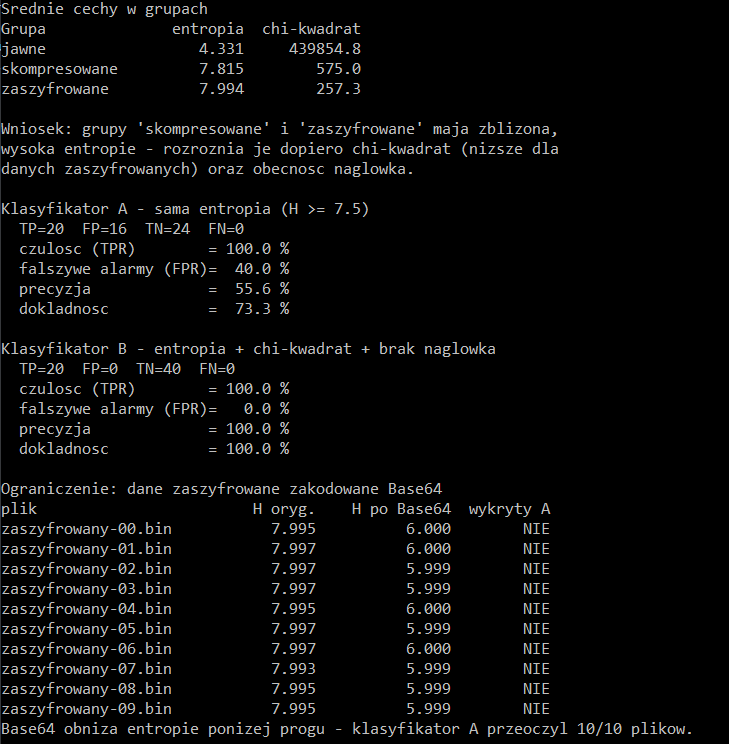
\includegraphics[width=0.72\textwidth]{rysunki/r6-entropia.png}
\caption{Wynik działania skryptu \kod{r6-entropia.py} na zbiorze testowym}
\label{rys:entropia}
\end{figure}

Skrypt sprawdzał również wpływ kodowania Base64, stosowanego do przesyłania danych binarnych w~kanałach tekstowych (np. w~poczcie elektronicznej lub w~treści żądań HTTP). Dziesięć pierwszych plików zaszyfrowanych zakodowano w~Base64 i~ponownie wyznaczono entropię. We wszystkich przypadkach spadła ona z~7,993--7,997 do 5,999--6,000~bitów na bajt, ponieważ alfabet Base64 liczy 64~znaki, a~$\log_2 64 = 6$. Wszystkie 10 plików znalazło się poniżej progu entropii i~nie zostało wykrytych. Dotyczy to obu klasyfikatorów, ponieważ warunek entropii jest częścią każdego z~nich.

\subsection*{Pliki rzeczywiste}

Zbiór testowy modeluje dane zaszyfrowane jako dane losowe bez nagłówka. Aby sprawdzić klasyfikatory na rzeczywistych plikach zaszyfrowanych, uruchomiono je na dziewięciu plikach utworzonych w~rozdziale~\ref{ch:gpu}: trzech kontenerach VeraCrypt, pięciu bazach KeePass i~archiwum 7-Zip z~hasłem. Do listy rozpoznawanych nagłówków dodano sygnaturę formatu KDBX. Pliki analizowano w~całości, ponieważ żaden nie przekraczał przyjętej wielkości próbki (8~MiB). Wyniki zawiera tabela~\ref{tab:realne}.

\begin{table}[htbp]
\centering\small
\begin{tabular}{@{}lrrrlcc@{}}
\toprule
\textbf{Plik} & \textbf{Rozmiar [B]} & \textbf{$H$} & \textbf{$\chi^2$} & \textbf{Nagłówek} & \textbf{A} & \textbf{B} \\
\midrule
\kod{kp-aeskdf-kdbx31.kdbx} & 1\,390 & 7,8442 & 342,7  & KDBX & tak & nie \\
\kod{kp-aeskdf-kdbx4.kdbx}  & 1\,656 & 7,7857 & 956,9  & KDBX & tak & nie \\
\kod{kp-argon2d-64.kdbx}    & 1\,990 & 7,7553 & 1\,602,7 & KDBX & tak & nie \\
\kod{kp-argon2d-256.kdbx}   & 1\,526 & 7,6398 & 2\,059,0 & KDBX & tak & nie \\
\kod{kp-argon2d-1024.kdbx}  & 1\,846 & 7,7346 & 1\,706,1 & KDBX & tak & nie \\
\kod{test-7zip.7z}          & 5\,263 & 7,9544 & 337,2  & 7z   & tak & nie \\
\kod{vc-sha512-pim1.hc}     & 2\,097\,152 & 7,9999 & 267,1 & -- & tak & tak \\
\kod{vc-sha512-pim250.hc}   & 2\,097\,152 & 7,9999 & 248,7 & -- & tak & tak \\
\kod{vc-sha512-pim500.hc}   & 2\,097\,152 & 7,9999 & 283,0 & -- & tak & tak \\
\bottomrule
\end{tabular}
\caption{Klasyfikatory A i~B na rzeczywistych plikach zaszyfrowanych}
\label{tab:realne}
\end{table}

Klasyfikator A uznał za zaszyfrowane wszystkie 9 plików, a~klasyfikator B -- tylko 3 kontenery VeraCrypt. Kontenery te nie mają nagłówka rozpoznawalnego po sygnaturze, a~ich rozkład bajtów odpowiada danym losowym. Bazy KeePass i~archiwum 7-Zip zaczynają się sygnaturą swojego formatu, więc klasyfikator B odrzucił je już na podstawie nagłówka; ponadto wszystkie miały statystykę $\chi^2$ powyżej progu. Wynik pokazuje, że warunek braku nagłówka, który na zbiorze testowym eliminował fałszywe alarmy dla archiwów, powoduje jednocześnie pominięcie zaszyfrowanych formatów mających własny nagłówek. Formaty takie wymagają osobnej reguły systemu DLP, uwzględniającej budowę formatu: baza KeePass jest zawsze zaszyfrowana, więc wystarcza sama sygnatura, natomiast archiwum 7-Zip może, ale nie musi być zaszyfrowane.

% ---------------------------------------------------------------------
\section{Weryfikacja skuteczności systemu}\label{sec:weryfikacja}

Tabela~\ref{tab:pokrycie} zestawia zagrożenia zbadane w~rozdziałach~\ref{ch:ataki} i~\ref{ch:gpu} z~mechanizmami, które je ograniczają. Część zagrożeń jest wykrywana przez warstwy detekcji opisane w~tym rozdziale, a~części zapobiegają poprawione konfiguracje i~mechanizmy kryptograficzne zbadane wcześniej.

\begin{table}[htbp]
\centering\small
\begin{tabularx}{\textwidth}{@{}>{\raggedright\arraybackslash}p{3.3cm} >{\raggedright\arraybackslash}p{3.6cm} L@{}}
\toprule
\textbf{Zagrożenie} & \textbf{Mechanizm} & \textbf{Wynik weryfikacji} \\
\midrule
podszycie w~ARP & detekcja: inspektor \kod{arp\_spoof} & 3 z~3 ramek wykryte; 3 fałszywe alarmy 112:1 na zwykłym ruchu \\
sesja z~przestarzałą wersją TLS & detekcja: reguły 1000010--1000012 & 6 z~6 sesji wykryte, 0 fałszywych alarmów na 9 sesjach poprawnych \\
& zapobieganie: wyłączenie wersji starszych niż TLS~1.2 & serwer utwardzony przyjmuje tylko TLS~1.2 i~1.3 (podrozdział~\ref{sec:tlsneg}) \\
słaby zestaw szyfrów & detekcja: reguła 1000013 & 6 z~6 sesji wykryte, 0 fałszywych alarmów \\
modyfikacja ciasteczka & zapobieganie: tryb AES-GCM & 0 z~400 modyfikacji przyjętych (podrozdziały~\ref{sec:ctr}, \ref{sec:cbc}); brak detekcji w~warstwie sieciowej \\
podpis żądania API & zapobieganie: HMAC-SHA-256 & konstrukcja odporna na atak przedłużenia (podrozdział~\ref{sec:lenext}) \\
łamanie hasła offline & zapobieganie: funkcja memory-hard z~dużą pamięcią & przewaga GPU nad CPU spada do 2,1$\times$ przy 1~GiB (podrozdział~\ref{sec:gpu-memory}) \\
eksfiltracja danych zaszyfrowanych & detekcja: klasyfikator B & zbiór testowy: 20 z~20 wykryte, 0 z~40 fałszywych alarmów; pliki rzeczywiste: 3 z~9 wykryte \\
\bottomrule
\end{tabularx}
\caption{Zagrożenia zbadane w~pracy i~mechanizmy, które je ograniczają}
\label{tab:pokrycie}
\end{table}

Warstwa sieciowa wykryła wszystkie badane zdarzenia: próbę podszycia w~ARP oraz wszystkie sesje z~przestarzałą wersją protokołu i~słabym zestawem szyfrów. Nie zgłosiła żadnego alarmu dla sesji serwera utwardzonego. Jej słabym punktem są alarmy 112:1, które stanowiły wszystkie 3 fałszywe alarmy w~nagraniu \kod{r4.pcap}. Warstwa danych w~wariancie B rozdzieliła bezbłędnie dane zaszyfrowane i~skompresowane w~zbiorze testowym, podczas gdy klasyfikator oparty na samej entropii dawał 40\% fałszywych alarmów. Na plikach rzeczywistych wykrył jednak tylko kontenery bez nagłówka.

Warstwy obejmują różne etapy ataku. Warstwa sieciowa wykrywa przygotowanie i~przeprowadzenie ataku w~sieci, czyli uzyskanie pozycji pośrednika i~zestawienie słabej sesji. Warstwa danych wykrywa próbę wyprowadzenia danych. Żadna z~nich nie wykrywa ataków na integralność danych aplikacji (podrozdziały~\ref{sec:ctr}--\ref{sec:lenext}) ani łamania haseł offline, które odbywa się poza siecią organizacji. Przed tymi zagrożeniami chronią wyłącznie mechanizmy zapobiegawcze: uwierzytelnione szyfrowanie, kod HMAC i~funkcje memory-hard. Uzasadnia to podejście wielowarstwowe, w~którym detekcja uzupełnia poprawną konfigurację kryptograficzną, a~nie ją zastępuje.

% ---------------------------------------------------------------------
\section{Ograniczenia rozwiązania}\label{sec:ograniczenia}

Weryfikacja ujawniła następujące ograniczenia, wynikające z~uzyskanych wyników lub z~budowy mechanizmów:
\begin{enumerate}
  \item \textbf{Kodowanie Base64 ukrywa dane zaszyfrowane.} Obniża ono entropię do około 6~bitów na bajt, przez co oba klasyfikatory przeoczyły 10 z~10 zakodowanych plików. Przed analizą entropii należałoby zdekodować typowe kodowania transportowe.
  \item \textbf{Formaty zaszyfrowane z~nagłówkiem nie są wykrywane przez klasyfikator B.} Bazy KeePass i~archiwum 7-Zip zostały odrzucone na podstawie nagłówka. Takie formaty wymagają osobnej reguły opartej na sygnaturze.
  \item \textbf{O~odróżnieniu części archiwów decyduje wyłącznie nagłówek.} Pięć archiwów gzip spełniło warunki entropii i~$\chi^2$. Dane skompresowane pozbawione nagłówka zostałyby więc uznane za zaszyfrowane.
  \item \textbf{Próg $\chi^2$ dopuszcza pominięcia.} Przy progu równym kwantylowi 0,95 około 5\% plików o~rozkładzie jednostajnym przekracza próg i~zostaje pominiętych. W~badanym zbiorze żaden z~20 plików zaszyfrowanych nie przekroczył progu, ale przy większej liczbie plików pominięcia są oczekiwane. Dla bardzo małych plików liczba bajtów przypadająca na jedną z~256 wartości jest mała, przez co rozkład statystyki słabiej zgadza się z~rozkładem chi-kwadrat.
  \item \textbf{Alarm 112:1 generuje fałszywe alarmy na zwykłym ruchu.} Zgłasza on każde zapytanie ARP typu unicast, w~tym zapytania wysyłane przy odświeżaniu tablicy sąsiadów. Alarm 112:4 działa tylko dla adresów wpisanych do wzorca, a~alarmy w~formacie \kod{alert\_fast} nie zawierają adresów, więc ich analiza wymaga sięgnięcia do nagrania.
  \item \textbf{Reguły TLS zależą od położenia pól w~pakiecie.} Zakładają, że rekord ServerHello zaczyna się na początku analizowanych danych (opcja \kod{offset 0}); w~nagraniu warunek ten był spełniony dla wszystkich 15 komunikatów. Reguła 1000013 jest ponadto heurystyką, która może dać fałszywy alarm przy przypadkowym wystąpieniu bajtów \kod{0xC014} w~polach losowych.
  \item \textbf{Reguła kontrolna ruchu HTTP nie zadziałała.} Plik reguł zawiera regułę kontrolną (sid 1000001) wykrywającą żądania \kod{GET} do aplikacji testowej. Mimo 827 takich żądań w~nagraniu nie wygenerowała ona żadnego alarmu. Przyczyny nie ustalono; reguła nie należy do ocenianej detekcji.
  \item \textbf{Zakres weryfikacji.} Obie warstwy weryfikowano offline, na nagraniach z~jednego stanowiska laboratoryjnego i~na syntetycznym zbiorze 60 plików uzupełnionym 9 plikami rzeczywistymi. Wyniki nie obejmują pracy czujnika na ruchu na żywo ani skuteczności na dużych, zróżnicowanych zbiorach danych.
\end{enumerate}
